\textit{Response.} 

\begin{enumerate}[a)]
	\item We begin by writing the model in matrix form
	
	\begin{equation}
		\dv{\va{u}}{t} = \vb{F}\,\va{u} + \vb{\Sigma}\,\dot{\va{W}},
	\end{equation}
	
	where
	
	\begin{equation}
		\va{u} = \mqty[u_1 \\ u_2],\qquad \vb{F} = \mqty[F_{11} & F_{12} \\ F_{21} & F_{22}],\qquad \vb{\Sigma} = \mqty[\sigma_1 & 0 \\ 0 & \sigma_2],\qquad \dot{\va{W}} = \mqty[\dot{W}_1 \\ \dot{W}_{2}].
	\end{equation}
	
	Since the model is linear with Gaussian noise, we know that the equilibrium distribution is a unique Gaussian. Hence, the equilibrium distribution is given by solving the equations

	\begin{subequations}
		\begin{equation}
			\dv{\gang{\va{u}}_{eq}}{t} = 0,
		\end{equation}
		\begin{equation}
			\dv{\cov{\va{u}}{\va{u}}_{eq}}{t} = 0.
		\end{equation}	
	\end{subequations}
	
	To examine the first of these equations, we note that we may write the solution to the differential equation for $\gang{\va{u}}$ explicitly
	
	\begin{equation}
		\dv{\gang{\va{u}}}{t} = \vb{F}\,\gang{\va{u}} \qquad \impl \qquad \gang{\va{u}} = \vb{Q}\,\mqty[e^{\lambda_1\,t} & 0 \\ 0 & e^{\lambda_2\,t}]\,\vb{Q}^{-1}\,\gang{\va{u}}_0,
	\end{equation}
	
	where $\vb{Q}$ is the eigenvector matrix of $\vb{F}$, $\lambda_1$ and $\lambda_2$ are the eigenvalues of $\vb{F}$, and $\gang{\va{u}}_0$ is the initial mean of $\va{u}$. Notice that we assumed $\vb{F}$ to be diagonalizable (to utilize the eigenvalue decomposition) and that the mean is finite for large $t$ if and only if the real part of the eigenvalues of $\vb{F}$ are non-positive. If the real part of $\lambda_1$ and $\lambda_2$ are zero and their imaginary part is non-zero, then $\gang{u_1}$ and $\gang{u_2}$ will forever oscillate and there will be no equilibrium mean. On the other hand, if the real part of $\lambda_1$ and $\lambda_2$ are negative then $\gang{u_1}$ and $\gang{u_2}$ will always decay toward zero and thus the equilibrium mean will exist, i.e., either the real part of the eigenvalues of $\vb{F}$ must be negative or the eigenvalues of $\vb{F}$ must be zero. Since the eigenvalues of $\vb{F}$ are given by
	
	\begin{equation}
		\lambda = \frac{1}{2}\,\gpr{\gpr{F_{11} + F_{22}} \pm \sqrt{\gpr{F_{11} - F_{22}}^2 - 4\,F_{12}\,F_{21}}},
	\end{equation}
	
	this is equivalent to the condition that $\tr{\vb{F}} = F_{11} + F_{22} \leq 0$. Further, we have that $\det{\vb{F}} \geq 0$
	
	Now, to calculate the the equilibrium covariance it is easier to calculate the evolutions of $\vr{u_1}$, $\vr{u_2}$, and $\cov{u_1}{u_2}$ individually. We begin by stating the evolution of $\gang{u_1}$ and $\gang{u_2}$ in scalar form
	
	\begin{subequations}
		\begin{equation}
			d\gang{u_1} = \gpr{F_{11}\,\gang{u_1} + F_{12}\,\gang{u_2}}\,dt,
		\end{equation}
		\begin{equation}
			d\gang{u_2} = \gpr{F_{21}\,\gang{u_1} + F_{22}\,\gang{u_2}}\,dt.
		\end{equation}
	\end{subequations}
	
	To calculate the scalar variances and covariance, we note It\^{o}'s formula for a multivariate scalar function
	
	\begin{equation}
		d\func{f}{x,\ y} = \pdv{f}{x}\,dx + \pdv{f}{y}\,dy + \frac{1}{2}\,\gpr{\pdv[2]{f}{x}\,\gpr{dx}^2 + 2\,\pdv{f}{x}{y}\,dx\,dy + \pdv[2]{f}{y}\,\gpr{dy}^2}.
	\end{equation}
	
	Specifically, for $\func{f}{u_1,\ u_2}$ we have
	
	\begin{align}
		d\func{f}{u_1,\ u_2} &= \pdv{f}{u_1}\,du_1 + \pdv{f}{u_2}\,du_2 + \frac{1}{2}\,\gpr{\pdv[2]{f}{u_1}\,\gpr{du_1}^2 + 2\,\pdv{f}{u_1}{u_2}\,du_1\,du_2 + \pdv[2]{f}{u_2}\,\gpr{du_2}^2} \nonumber \\
			&= \pdv{f}{u_1}\,\gpr{\gpr{F_{11}\,u_1 + F_{12}\,u_2}\,dt + \sigma_1\,dW_1} + \pdv{f}{u_2}\,\gpr{\gpr{F_{21}\,u_1 + F_{22}\,u_2}\,dt + \sigma_2\,dW_2} \nonumber \\
				&\qquad + \frac{1}{2}\,\left( \pdv[2]{f}{u_1}\,\gpr{\gpr{F_{11}\,u_1 + F_{12}\,u_2}\,dt + \sigma_1\,dW_1}^2 \right. \nonumber \\
				&\qquad\qquad \phantom{+ \frac{1}{2}} + \left. 2\,\pdv{f}{u_1}{u_2}\,\gpr{\gpr{F_{11}\,u_1 + F_{12}\,u_2}\,dt + \sigma_1\,dW_1} \right. \nonumber \\
				&\qquad\qquad\qquad \phantom{+ \frac{1}{2}} \cdot \left. \gpr{\gpr{F_{21}\,u_1 + F_{22}\,u_2}\,dt + \sigma_2\,dW_2} \right. \nonumber \\
				&\qquad\qquad \phantom{+ \frac{1}{2}} + \left. \pdv[2]{f}{u_2}\,\gpr{\gpr{F_{21}\,u_1 + F_{22}\,u_2}\,dt + \sigma_2\,dW_2}^2 \right) \nonumber \\
			&= \gpr{\pdv{f}{u_1}\,\gpr{F_{11}\,u_1 + F_{12}\,u_2} + \pdv{f}{u_2}\,\gpr{F_{21}\,u_1 + F_{22}\,u_2} + \frac{1}{2}\,\gpr{\sigma_1^2\,\pdv[2]{f}{u_1} + \sigma_2^2\,\pdv[2]{f}{u_2}}}\,dt \nonumber \\
			&\qquad + \sigma_1\,\sigma_2\,\pdv{f}{u_1}{u_2}\,dW_1\,dW_2 + \sigma_1\,\pdv{f}{u_1}\,dW_1 + \sigma_2\,\pdv{f}{u_2}\,dW_2
	\end{align}
	
	where we have utilized the fact that $\gpr{dW_1}^2 = \gpr{dW_2}^2 = \func{o}{dt}$, and that $dt^2$, $dt\,dW_1$, and $dt\,dW_2$ go to zero faster than $dt$ in the limit $dt \to 0$.
	
	Now, to calculate the evolution of $\vr{u_1}$ we need only calculate $d\gang{u_1^2}$
	
	\begin{align}
		d\gang{u_1^2} &= \gang{\gpr{2\,u_1\,\gpr{F_{11}\,u_1 + F_{12}\,u_2} + 0 + \frac{1}{2}\,\gpr{2\,\sigma_1^2 + 0}}\,dt + 0 + 2\,\sigma_1\,u_1\,dW_1 + 0} \nonumber \\
			&= \gpr{2\,\gpr{F_{11}\,\gang{u_1^2} + F_{12}\,\gang{u_1\,u_2}} + \sigma_1^2}\,dt,
	\end{align}
	
	where we have utilize the fact that $u_1$ and $dW_1$ are independent. We may thus obtain
	
	\begin{align}
		d\vr{u_1} &= d\gang{u_1^2} - 2\,\gang{u_1}\,d\gang{u_1} \nonumber \\
			&= \gpr{2\,\gpr{F_{11}\,\gang{u_1^2} + F_{12}\,\gang{u_1\,u_2}} + \sigma_1^2}\,dt - 2\,\gpr{F_{11}\,\gang{u_1}^2 + F_{12}\,\gang{u_1}\,\gang{u_2}}\,dt \nonumber \\
			&= \gpr{2\,\gpr{F_{11}\,\vr{u_1} + F_{12}\,\cov{u_1}{u_2}} + \sigma_1^2}\,dt.
	\end{align}
	
	We may similarly show that the variance of $u_2$ is governed by a similar equation
	
	\begin{equation}
		d\vr{u_2} = \gpr{2\,\gpr{F_{21}\,\cov{u_1}{u_2} + F_{22}\,\vr{u_2}} + \sigma_2^2}\,dt.
	\end{equation}
	
	Lastly, to obtain the evolution of the covariance of $u_1$ and $u_2$ we first calculate $d\gang{u_1\,u_2}$
	
	\begin{align}
		d\gang{u_1\,u_2} &= \left\langle \gpr{u_2\,\gpr{F_{11}\,u_1 + F_{12}\,u_2} + u_1\,\gpr{F_{21}\,u_1 + F_{22}\,u_2} + \frac{1}{2}\,\gpr{0 + 0}}\,dt \right. \nonumber \\
				&\qquad  + \left.\sigma_1\,\sigma_2\,dW_1\,dW_2 + \sigma_1\,u_2\,dW_1 + \sigma_2\,u_1\,dW_2 \right\rangle \nonumber \\
			&= \gpr{\gpr{F_{11} + F_{22}}\,\gang{u_1\,u_2} + F_{21}\,\gang{u_1^2} + F_{12}\,\gang{u_2^2}}\,dt,
	\end{align}
	
	where we have utilized the fact that $dW_1$ and $dW_2$ are independent, $u_2$ and $dW_1$ are independent, and $u_1$ and $dW_2$ are independent. The covariance of $u_1$ and $u_2$ is therefore governed by
	
	\begin{align}
		d\cov{u_1}{u_2} &= d\gang{u_1\,u_2} - \gpr{\gang{u_2}\,d\gang{u_1} + \gang{u_1}\,d\gang{u_2}} \nonumber \\
			&= \gpr{\gpr{F_{11} + F_{22}}\,\gang{u_1\,u_2} + F_{21}\,\gang{u_1^2} + F_{12}\,\gang{u_2^2}}\,dt \nonumber \\
				&\qquad - \gpr{\gpr{F_{11}\,\gang{u_1}\,\gang{u_2} + F_{12}\,\gang{u_2}^2}\,dt  + \gpr{F_{21}\,\gang{u_1}^2 + F_{22}\,\gang{u_1}\,\gang{u_2}}\,dt} \nonumber \\
			&= \gpr{\gpr{F_{11} + F_{22}}\,\cov{u_1}{u_2} + F_{21}\,\vr{u_1} + F_{12}\,\vr{u_2}}\,dt.
	\end{align}
	
	We may now actually write the evolution of the covariance of $\va{u}$ in matrix form
	
	\begin{equation}
		\dv{\cov{\va{u}}{\va{u}}}{t} = \vb{F}\,\cov{\va{u}}{\va{u}} + \cov{\va{u}}{\va{u}}\,\vb{F}^T + \vb{\Sigma}^2,
	\end{equation}
	
	where we have utilized the symmetry of $\cov{\va{u}}{\va{u}}$. For this to reach some equilibrium value, we must have
	
	\begin{align}
		\dv{\cov{\va{u}}{\va{u}}_{eq}}{t} = \vb{F}\,\cov{\va{u}}{\va{u}}_{eq} + \cov{\va{u}}{\va{u}}_{eq}\,\vb{F}^T + \vb{\Sigma}^2 = \vb{0} \nonumber \\
		\qquad \impl \qquad \vb{F}\,\cov{\va{u}}{\va{u}}_{eq} + \cov{\va{u}}{\va{u}}_{eq}\,\vb{F}^T  = -\vb{\Sigma}^2.
	\end{align}
	
	With great effort, we may solve for $\vr{u_1}_{eq}$, $\vr{u_2}_{eq}$, and $\cov{u_1}{u_2}_{eq}$ explicitly in terms of $\vb{F}$ and $\vb{\Sigma}$ so long as the determinant of $\vb{F}$ is non-zero
	
	\begin{subequations}
		\begin{align}
			\vr{u_1}_{eq} &= -\frac{\sigma_1^2\,\gpr{\det{\vb{F}} + F_{22}^2} + \sigma_2^2\,F_{12}^2}{2\,\tr{\vb{F}}\,\det{\vb{F}}}, \\
			\vr{u_2}_{eq} &= -\frac{\sigma_1^2\,F_{21}^2 + \sigma_2^2\,\gpr{\det{\vb{F}} + F_{11}^2}}{2\,\tr{\vb{F}}\,\det{\vb{F}}}, \\
			\cov{u_1}{u_2}_{eq} &= \frac{\sigma_1^2\,F_{21}\,F_{22} + \sigma_2^2\,F_{11}\,F_{12}}{2\,\tr{\vb{F}}\,\det{\vb{F}}}.
		\end{align}
	\end{subequations}	
	
	As $\vr{u_1}$ and $\vr{u_2}$ must be positive, we also have that the trace of $\vb{F}$ must be negative. \textbf{In summary}, for the equilibrium distribution to exist, we must have $\tr{\vb{F}} = F_{11} + F_{22} < 0$ and $\det{\vb{F}} = F_{11}\,F_{22} - F_{12}\,F_{21} > 0$. Note that this also implies that $\gang{\va{u}}_{eq} = \va{0}$.
	
	\item Below we include a plot of the equilibrium probability denisty function (Figure~\ref{fig:1b_eq_pdf}), a single trajectory for 100 time-units (Figure~\ref{fig:1b_traj}), and the ensemble statistics calculated from 500 trajectories (Figure~\ref{fig:1b_ens_stats}). Each realization utilized a time-step size of $\Delta t = 0.1$.
	
	\begin{figure}[H]
		\centering
		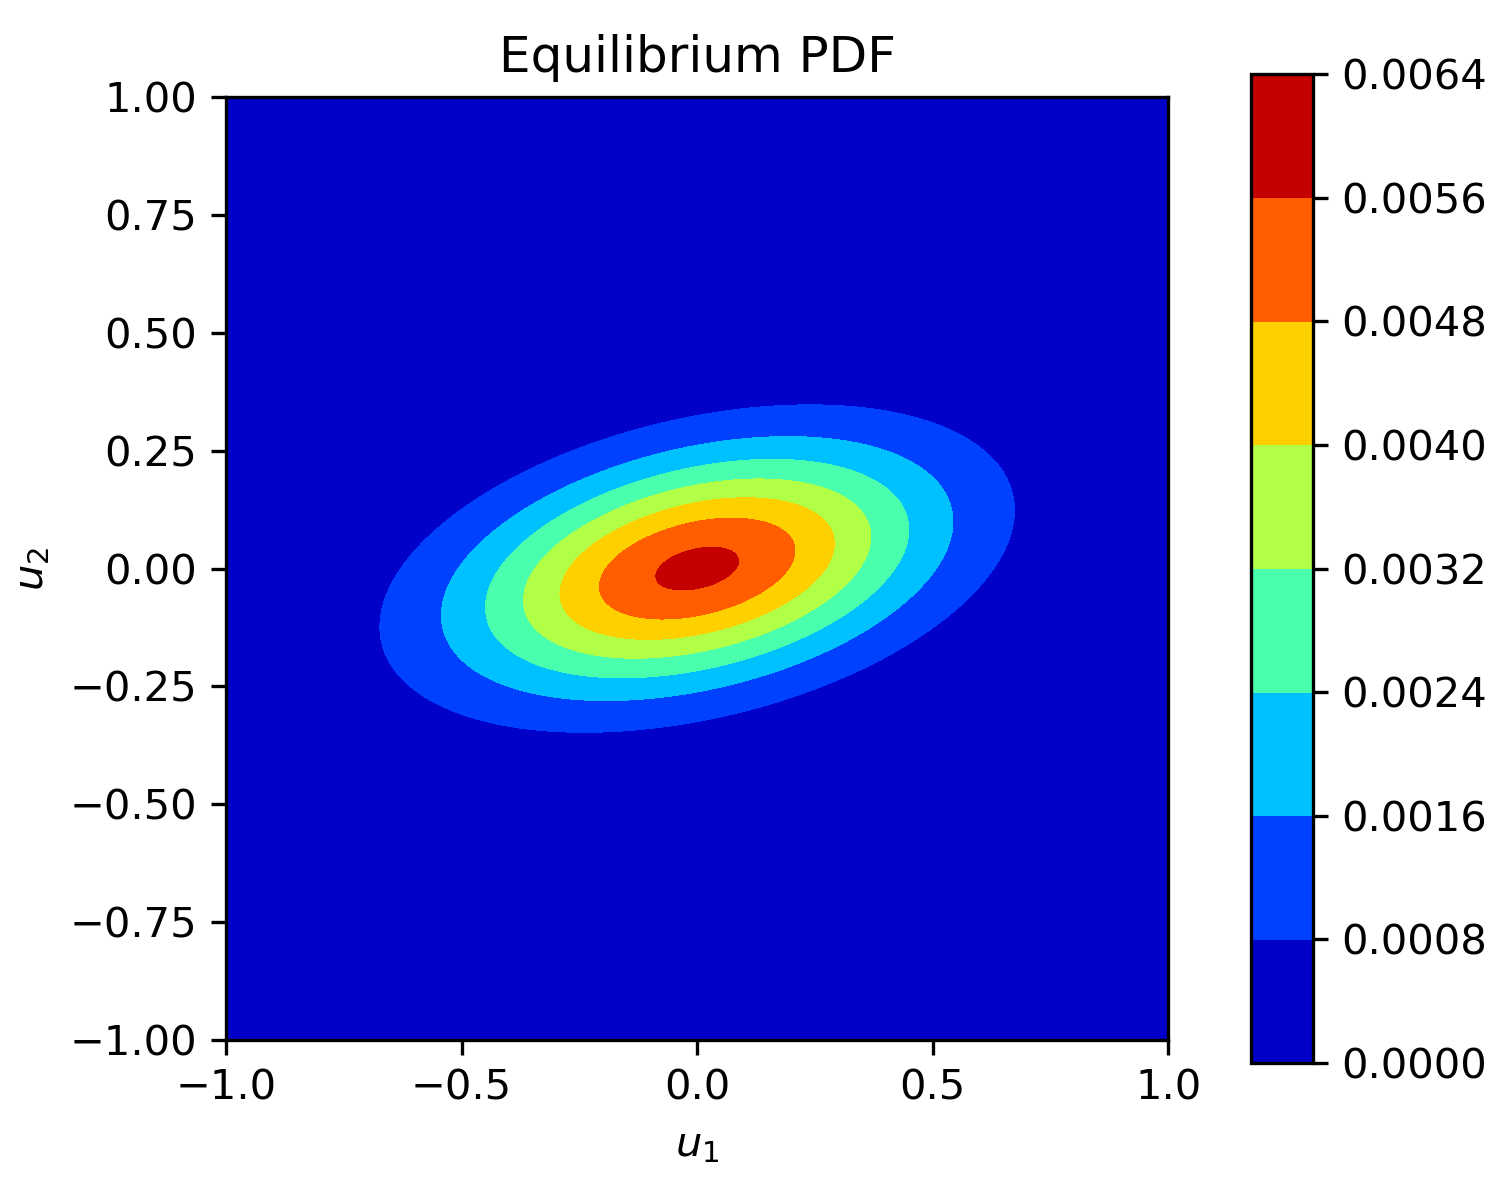
\includegraphics[width=0.75\textwidth]{../../src/1b_eq_pdf.png}
		\caption{The equilibrium probability density function for Eqs.~\ref{eqs:model_1} with the parameters $F_{11} = F_{22} = -1$, $F_{12} = -F_{21} = 0.5$, $\sigma_1 = 0.2$, and $\sigma_2 = 0.5$.}
		\label{fig:1b_eq_pdf}
	\end{figure}
	
	\begin{figure}[H]
		\centering
		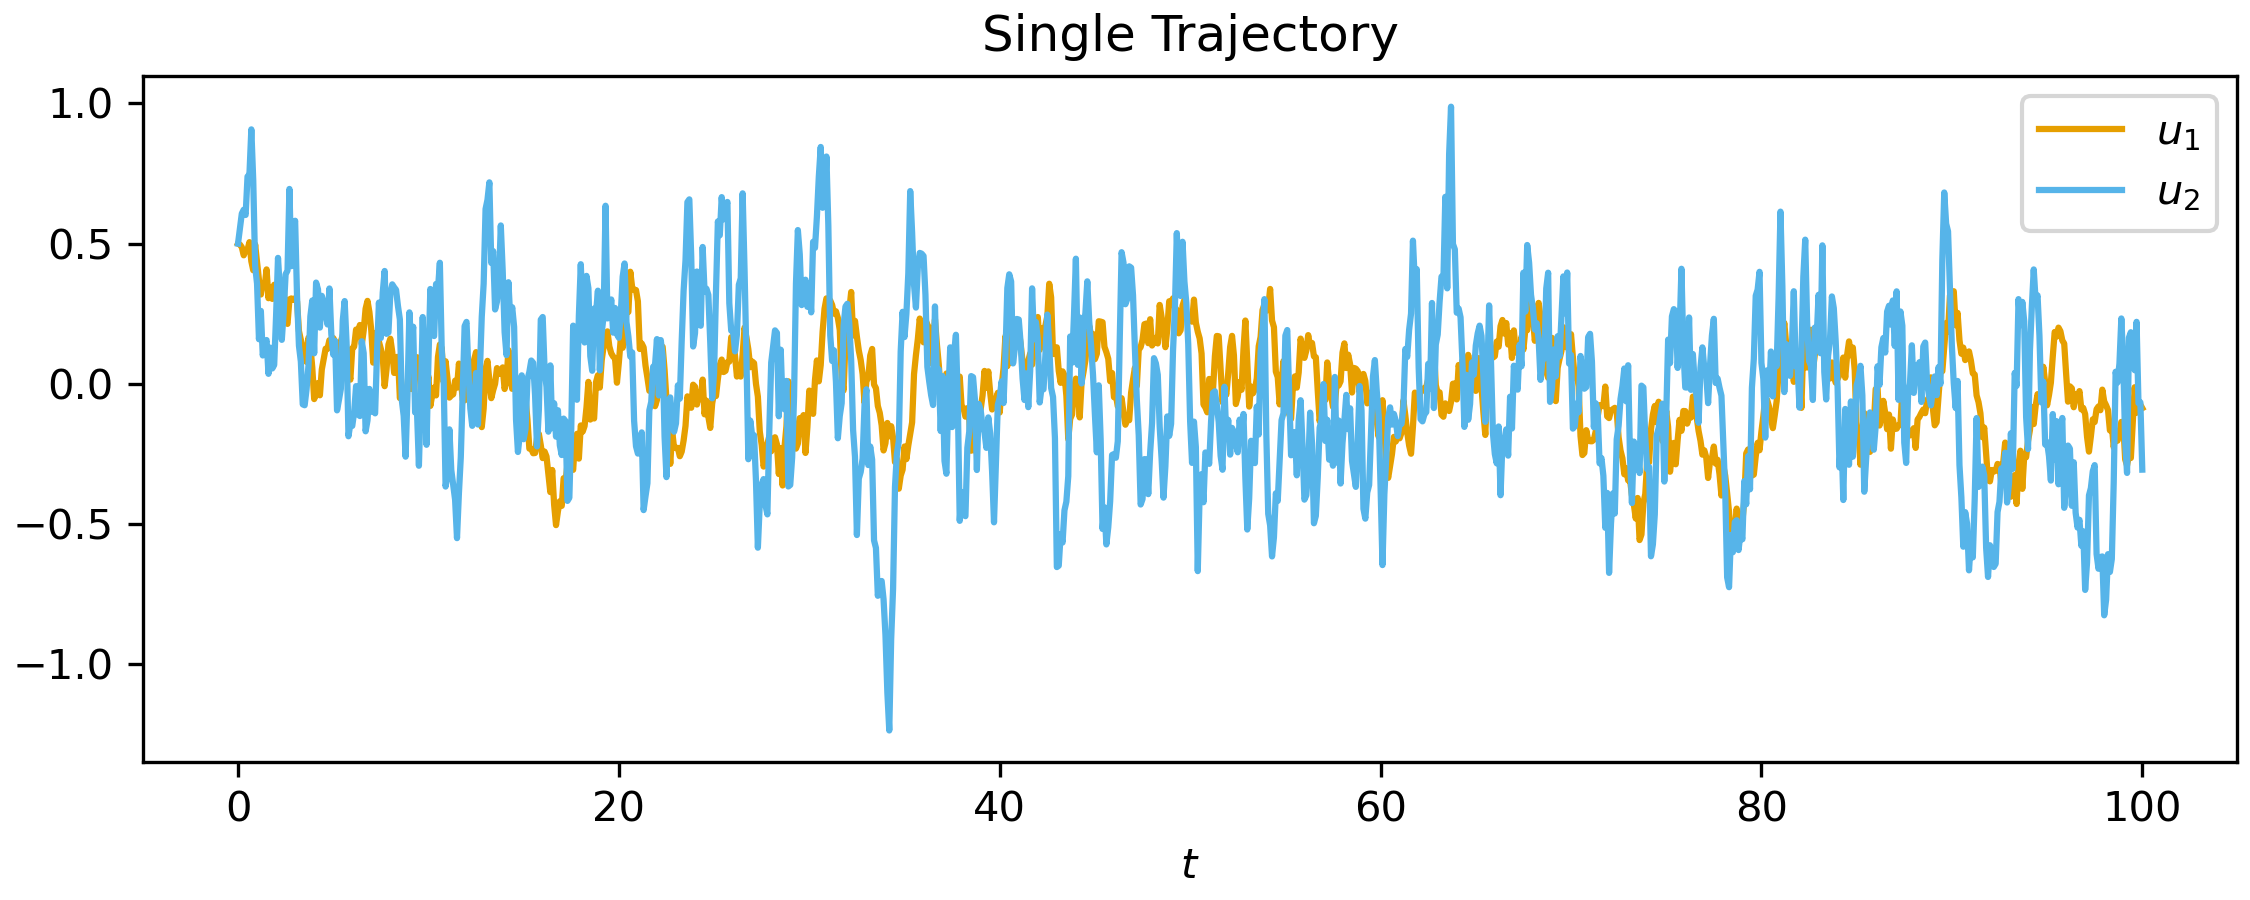
\includegraphics[width=0.75\textwidth]{../../src/1b_traj.png}
		\caption{A single realization of the model given by Eqs.~\ref{eqs:model_1} with the parameters $F_{11} = F_{22} = -1$, $F_{12} = -F_{21} = 0.5$, $\sigma_1 = 0.2$, and $\sigma_2 = 0.5$, with initial condition $u_1 = u_2 = 0.5$.}
		\label{fig:1b_traj}
	\end{figure}
	
	\begin{figure}[H]
		\centering
		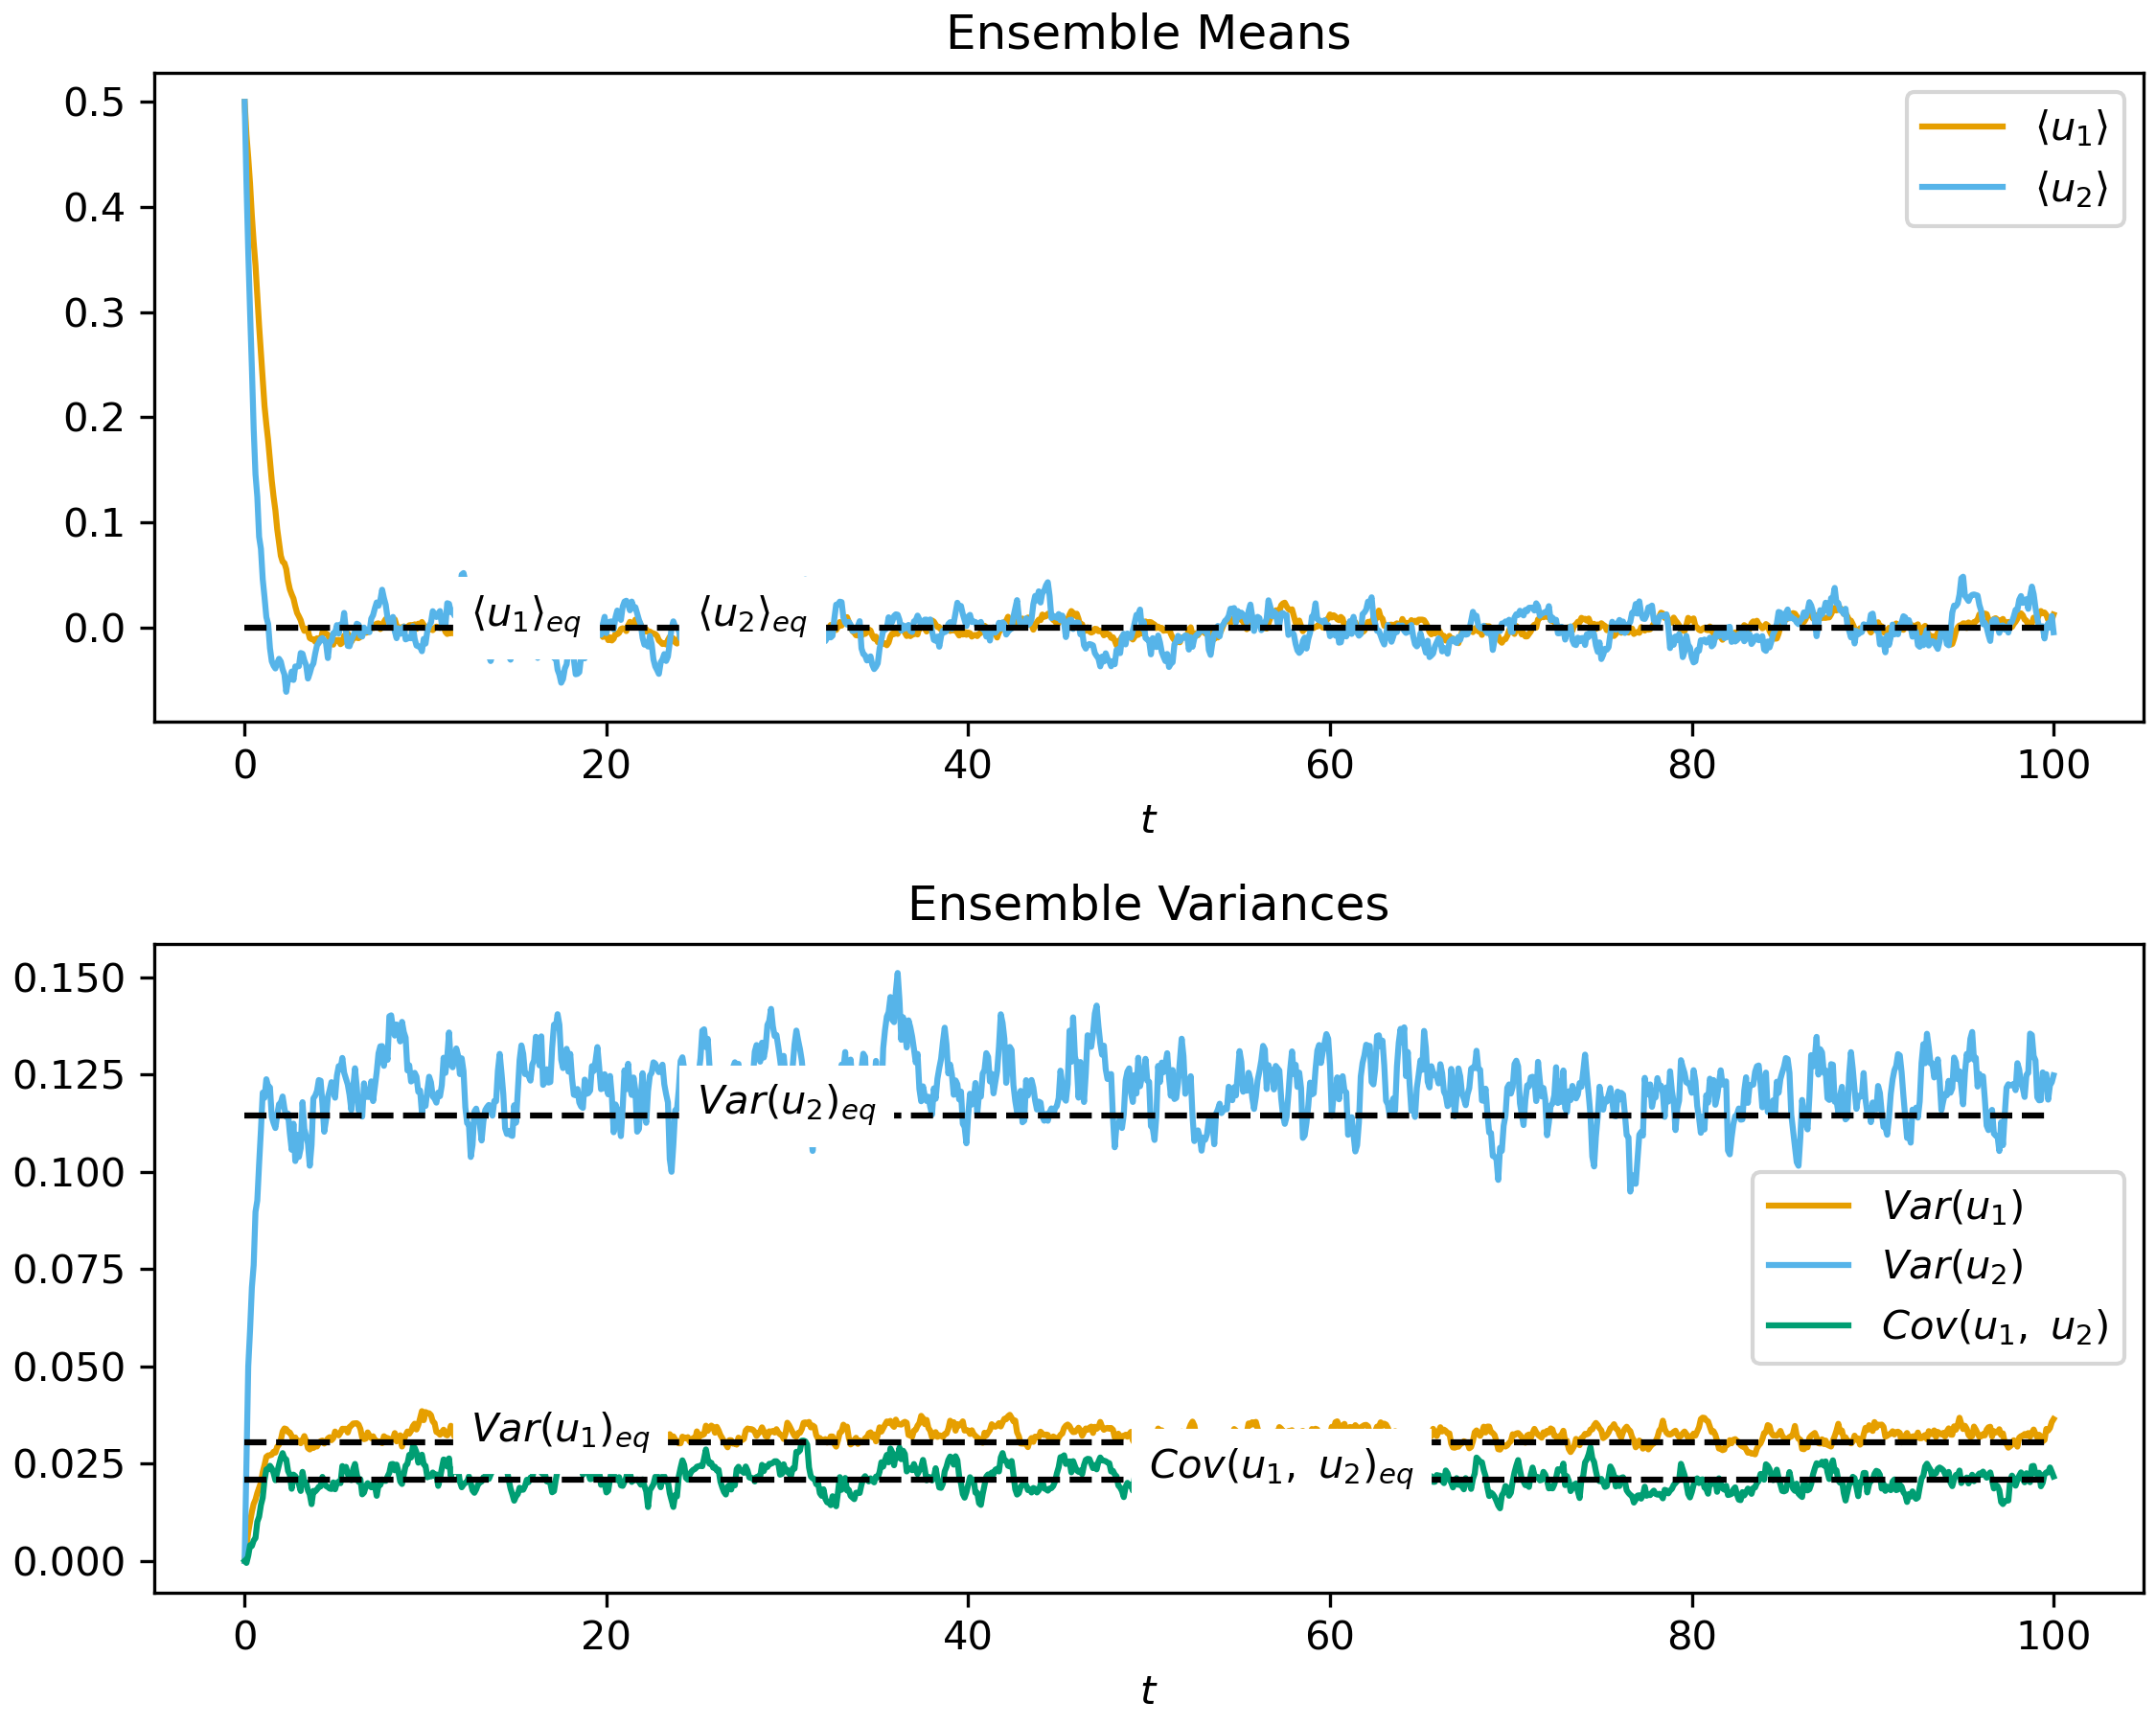
\includegraphics[width=0.75\textwidth]{../../src/1b_ens_stats.png}
		\caption{The ensemble statistics for 500 realizations of the model given by Eqs.~\ref{eqs:model_1} with the parameters $F_{11} = F_{22} = -1$, $F_{12} = -F_{21} = 0.5$, $\sigma_1 = 0.2$, and $\sigma_2 = 0.5$, with initial condition $u_1 = u_2 = 0.5$ for each realization. The equilibrium values for the means and variances are given by the dashed horizontal black lines.}
		\label{fig:1b_ens_stats}
	\end{figure}
	
	Source code is available from the GitHub repository
	
	\begin{center}
		\url{https://github.com/jasonltorchinsky/MATH833_HW/releases/tag/hw3}
	\end{center}

	and is given in Appendix~\ref{app:code_1b}. In short, the code takes a input parameters \texttt{-{-}F\_11}, \texttt{-{-}F\_12}, \texttt{-{-}F\_21}, \texttt{-{-}F\_12}, \texttt{-{-}sigma\_1}, and \texttt{-{-}sigma\_2} which correspond to $F_{11}$, $F_{12}$, $F_{21}$, $F_{22}$, $\sigma_1$, and $\sigma_2$, respectively. The code then calculates the equilibrium distribution from the analytic formulas derived in part a), simulates 500 indivual realizations of Eqs.~\ref{eqs:model_1} using the Euler--Maruyama method, and plots a single trajectory along with the statistics across all 500 realizations.
	
	\item We begin by rewriting the system model in a discretized form as a matrix equation
	
	\begin{equation}
		\va{u}_{k+1} = \gpr{\vb{\mathcal{I}} + h\,\vb{F}}\,\va{u}_{k} + \sqrt{h}\,\vb{\Sigma}\,\va*{\xi}_{k+1}
	\end{equation}		
	
	where $k$ indexes the time-step, $\vb{\mathcal{I}}$ is the identity matrix, $h$ is the time-step size (e.g., $h = 0.1$ in the realizations in part b))m and $\va*{\xi}_{k+1}$ is a vector of independent zero-mean unit-variance Gaussian noise.	We also write the observation model in discretized form as a matrix equation

	\begin{equation}
		\va{v}_{k+1} = \vb{G}\,\va{u} + \vb{\Sigma}^{o}\,\va*{\zeta}_{k+1}
	\end{equation}
		
	where 
	
	\begin{equation}
		\va{v} = \mqty[v_1 \\ v_2],\qquad \vb{G} = \mqty[g_1 & 0 \\ 0 & g_2],\qquad \vb{\Sigma}^{o} = \mqty[\sigma_1^{o} & 0 \\ 0 & \sigma_2^{o}],
	\end{equation}
	
	and $\va*{\zeta}_{k+1}$ is a vector of independent zero-mean unit-variance Gaussian noise.
	
	The prior mean $\overline{\va{u}}_{k+1 \vert k}$ and prior covariance $\vb{\Sigma}_{k+1 \vert k}$ of the Kalman filter is given by
	
	\begin{subequations}
		\begin{equation}
			\overline{\va{u}}_{k+1 \vert k} = \gpr{\vb{\mathcal{I}} + h\,\vb{F}}\,\overline{\va{u}}_{k \vert k},
		\end{equation}
		\begin{equation}
			\vb{\Sigma}_{k+1 \vert k} = \gpr{\vb{\mathcal{I}} + h\,\vb{F}}\,\vb{\Sigma}_{k \vert k}\,\gpr{\vb{\mathcal{I}} + h\,\vb{F}}^T + \vb{\Sigma},
		\end{equation}
	\end{subequations}
	
	and the posterior mean $\overline{\va{u}}_{k+1 \vert k+1}$ and posterior covariance $\vb{\Sigma}_{k+1 \vert k+1}$ of the Kalman filter is given by
	
	\begin{subequations}
		\begin{equation}
			\overline{\va{u}}_{k+1 \vert k+1} = \overline{\va{u}}_{k+1 \vert k} + \vb{K}_{k+1}\,\gpr{\va{v}_{k+1} - \vb{G}\,\overline{\va{u}}_{k+1 \vert k}},
		\end{equation}
		\begin{equation}
			\vb{\Sigma}_{k+1 \vert k+1} = \gpr{\vb{\mathcal{I}} - \vb{K}_{k+1}\,\vb{G}}\,\vb{\Sigma}_{k+1 \vert k},
		\end{equation}
	\end{subequations}
	
	where $\vb{K}_{k+1}$ is the Kalman gain matrix
	
	\begin{equation}
		\vb{K}_{k+1} = \vb{\Sigma}_{k+1 \vert k}\,\vb{G}^T\,\gpr{\vb{G}\,\vb{\Sigma}_{k+1 \vert k}\,\vb{G}^T + \vb{\Sigma}^{o}}^{-1}.
	\end{equation}
	
\end{enumerate}
